\chapter{Lecture 2: Topics in String Theory}

Leonard Susskind opens this lecture by stepping back from cosmology and returning, for a moment, to the special theory of relativity. The point of the reset is not historical; it is methodological. Before black-hole geometry appears, he wants one simple operational rule in hand: light rays are identified by the condition of zero proper time. The lecture then carries that rule into curved spacetime, writes down the Schwarzschild metric, separates the horizon from the singularity, and only after that classical groundwork pivots toward the quantum mechanics of black holes, hidden information, and the Bekenstein-Hawking area law. These notes follow Leonard Susskind's presentation closely, with conservative normalization of notation where needed, and are curated by LazyingArt LLC.

\section{Flat Spacetime, Proper Time, and Null Trajectories}

Susskind begins with the metric of flat spacetime. For two neighboring events separated by \(dt,dx,dy,dz\), the proper time is defined by
\begin{equation}
d\tau^2 = dt^2 - \frac{1}{c^2}\left(dx^2+dy^2+dz^2\right).
\end{equation}
This is the relativistic interval. The spatial terms come with the opposite sign from the time term, so the geometry is not the Euclidean geometry of an ordinary four-dimensional space.

The factor \(1/c^2\) is only a matter of units. One may always measure space and time in compatible units and set \(c=1\). Susskind keeps \(c\) for a moment in order to make the relation to the speed of light explicit, and then later suppresses it.

He also remarks that \(d\tau^2\) need not be positive for arbitrary pairs of neighboring events. If the spatial separation is sufficiently large compared with the time separation, the expression becomes negative. He does not pursue that point here. Instead, he turns immediately to the question that matters for the rest of the lecture: how do light rays move?

For a light ray moving purely along the \(x\)-direction, one may set \(dy=dz=0\). The defining rule is then
\begin{equation}
d\tau^2 = 0.
\end{equation}
This is the null condition. It is the lecture's first main principle, and it will survive every later change of geometry.

Applying it in flat spacetime gives
\begin{align}
0 &= dt^2 - \frac{1}{c^2}dx^2,\\
c^2dt^2 &= dx^2,\\
c\,dt &= \pm dx.
\end{align}
Dividing by \(dt\) yields
\begin{equation}
\frac{dx}{dt}=\pm c.
\end{equation}
The plus and minus signs correspond to right-moving and left-moving light rays.

What matters most is not the particular number \(c\), but the invariant statement behind it. In any metric, the way to determine the motion of light is to impose the condition that the interval along the trajectory vanish.

\section{From the Metric Tensor to Spherical Coordinates}

The lecture next broadens from special relativity to general relativity. In a general spacetime the geometry varies from place to place, and Susskind describes it by a metric tensor \(G_{\mu\nu}\). We will use the standard notation
\begin{equation}
ds^2 = g_{\mu\nu}\,dx^\mu dx^\nu.
\end{equation}
As usual, repeated indices are summed. This compact expression stands for all quadratic combinations of the coordinate differentials with their appropriate metric coefficients.

The logical rule for light does not change. In flat or curved spacetime alike, light rays are diagnosed by setting the interval to zero. Susskind alternates somewhat loosely between \(ds^2\), \(d\tau^2\), and the phrase ``proper time,'' but the intended content is the same: light moves on null trajectories.

Because the black hole to be studied is spherically symmetric, he then rewrites flat space in spherical coordinates. Instead of Cartesian coordinates \(x,y,z\), one uses a radial distance \(r\) and two angles. The angular geometry is summarized by the metric on the unit two-sphere,
\begin{equation}
d\Omega^2 = d\theta^2 + \sin^2\theta\,d\phi^2.
\end{equation}
If the sphere has radius \(r\), the corresponding angular line element is \(r^2d\Omega^2\). Thus, in units with \(c=1\), flat spacetime may be written as
\begin{equation}
d\tau^2 = dt^2 - \left(dr^2 + r^2 d\Omega^2\right).
\end{equation}
This is the baseline against which the black-hole metric will be presented.

\section{The Schwarzschild Metric as a Deformation of Flat Space}

At this point Susskind announces that he will not solve Einstein's equations. He simply writes down the metric of a black hole and inspects it. The lecture's rhythm matters here: the metric is introduced not as an isolated formula but as a deformation of the flat spherical line element just discussed.

The board at this moment is worth preserving because it shows that comparison explicitly.

\begin{figure}[h]
\centering

\includegraphics[width=0.82\textwidth]{lecture_02_figure_02.png}
\caption{Schwarzschild metric and radial black-hole sketch. The board places the flat spherical line element above the Schwarzschild deformation and isolates the factor \(1-\frac{2MG}{c^2r}\) together with the shorthand \(1-\frac{R_s}{r}\).}
\end{figure}

The upper line on the board repeats flat spacetime in spherical coordinates,
\begin{equation}
d\tau^2 = dt^2 - \left(dr^2 + r^2 d\Omega^2\right).
\end{equation}
The lower line introduces the Schwarzschild factor. If the mass of the black hole is \(m\), then its Schwarzschild radius is
\begin{equation}
R_s=\frac{2Gm}{c^2},
\end{equation}
so that the controlling factor may be written as
\begin{equation}
1-\frac{2Gm}{c^2r}=1-\frac{R_s}{r}.
\end{equation}

Following the lecture, we keep \(c\) explicit once and then mostly set \(c=1\). In standard form, the Schwarzschild metric is
\begin{equation}
d\tau^2
=
\left(1-\frac{2Gm}{c^2r}\right)dt^2
-
\frac{dr^2}{1-\frac{2Gm}{c^2r}}
-
r^2d\Omega^2.
\end{equation}

\begin{remark}
The screenshot strongly supports the structure of this equation, especially the repeated factor \(1-\frac{2MG}{c^2r}\) and the shorthand \(1-\frac{R_s}{r}\). However, the handwritten lower line is partly cropped and not every sign is perfectly legible. The formula above is therefore a cautious standard reconstruction, chosen because it matches the transcript and reduces to the flat spherical metric for \(r\to\infty\).
\end{remark}

That asymptotic check is the first thing Susskind emphasizes. Far from the black hole, \(R_s/r\ll 1\), so the coefficient of \(dt^2\) tends to \(1\), the denominator in the radial term tends to \(1\), and the metric becomes the flat spherical line element again.

The right-hand side of the board also carries a small unlabeled radial sketch. It is schematic rather than analytic, but it is useful evidence for the way spherical symmetry is being visualized.

\begin{figure}[h]
\centering
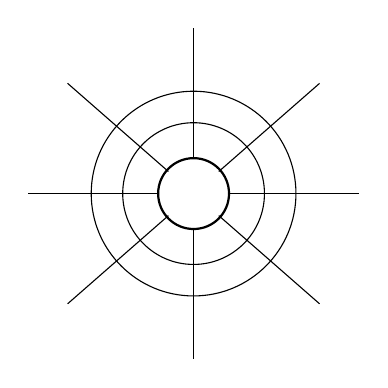
\begin{tikzpicture}[scale=1.0]
\draw[thick] (0,0) circle (0.45);
\draw (0,0) circle (0.9);
\draw (0,0) circle (1.3);
\draw (-2.1,0) -- (-0.45,0);
\draw (0.45,0) -- (2.1,0);
\draw (0,-2.1) -- (0,-0.45);
\draw (0,0.45) -- (0,2.1);
\draw (-1.6,-1.4) -- (-0.32,-0.28);
\draw (0.32,0.28) -- (1.6,1.4);
\draw (-1.6,1.4) -- (-0.32,0.28);
\draw (0.32,-0.28) -- (1.6,-1.4);
\end{tikzpicture}
\caption{A minimal redraw of the board's radial sketch. It should be read only as a schematic cue for spherical symmetry.}
\end{figure}

\section{Horizon, Singularity, and the Motion of Radial Light}

Once the metric is on the board, the lecture immediately asks where it looks strange. From here on Susskind suppresses \(c\) most of the time, so \(R_s=2Gm\). Two radii stand out:
\begin{equation}
r=2Gm
\qquad\text{and}\qquad
r=0.
\end{equation}
He is careful not to identify them with one another. The radius \(r=2Gm\) is the horizon. The radius \(r=0\) is the singularity. These are physically very different.

The difference is explained through tidal forces. At the horizon the tidal forces are finite, and for a sufficiently large black hole they are small. Falling through the horizon need not be violent at all. At the singularity, by contrast, tidal forces become infinite. That is the genuinely destructive place.

Only after making that distinction does Susskind ask again how light moves. Consider a radial light ray. Along such a ray the direction on the sphere is fixed, so
\begin{equation}
d\Omega^2=0.
\end{equation}
The rule is still the same as in flat spacetime: along a light ray, the proper time is zero. Applying that rule to the Schwarzschild metric gives
\begin{equation}
0=
\left(1-\frac{2Gm}{r}\right)dt^2
-
\frac{dr^2}{1-\frac{2Gm}{r}}.
\end{equation}
Rearranging,
\begin{equation}
\left(1-\frac{2Gm}{r}\right)dt^2
=
\frac{dr^2}{1-\frac{2Gm}{r}}.
\end{equation}
Multiplying through by the denominator and taking the square root yields
\begin{equation}
dr=\pm\left(1-\frac{2Gm}{r}\right)dt,
\end{equation}
and therefore
\begin{equation}
\frac{dr}{dt}=\pm\left(1-\frac{2Gm}{r}\right).
\end{equation}
The plus sign is the outgoing branch; the minus sign is the ingoing branch.

\begin{remark}
There is a short garbled stretch in the transcript during this manipulation, but the surrounding clean lines determine the algebra unambiguously. The reconstruction above is exactly the step needed to recover the light-ray equation that Susskind then discusses verbally.
\end{remark}

This is the one explicit property of the metric that the lecture promised to extract. Far from the black hole, \(2Gm/r\ll 1\), and the outgoing branch reduces to
\begin{equation}
\frac{dr}{dt}\approx 1,
\end{equation}
which is just the \(c=1\) version of ordinary light motion. Near the horizon,
\begin{equation}
\frac{dr}{dt}\to 0
\qquad\text{as}\qquad
r\to 2Gm.
\end{equation}
In these coordinates, outward-moving light rays slow down and finally stand still at the horizon.

Susskind then translates this into a spacetime picture in the \(t\)-\(r\) plane: time vertical, radius horizontal, and a vertical line marking \(r=2Gm\). Outgoing light rays start near \(45^\circ\) far away but become more and more vertical as they approach the horizon. Ingoing rays, drawn in the same coordinates, asymptotically approach the horizon.

\begin{figure}[h]
\centering
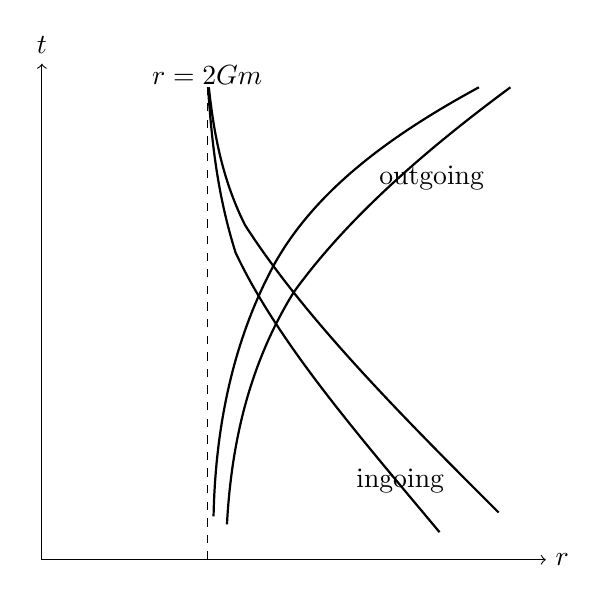
\begin{tikzpicture}[scale=1.0]
\draw[->] (0,0) -- (6.4,0) node[right] {$r$};
\draw[->] (0,0) -- (0,6.3) node[above] {$t$};

\draw[dashed] (2.1,0) -- (2.1,6.0);
\node at (2.1,6.15) {$r=2Gm$};

\draw[thick]
(2.18,0.55) .. controls (2.20,1.55) and (2.38,2.7) .. (2.95,3.75)
.. controls (3.45,4.65) and (4.35,5.35) .. (5.55,6.0);

\draw[thick]
(2.35,0.45) .. controls (2.40,1.35) and (2.58,2.4) .. (3.2,3.4)
.. controls (3.85,4.3) and (4.8,5.15) .. (5.95,6.0);

\draw[thick]
(5.8,0.6) .. controls (4.6,1.8) and (3.35,3.05) .. (2.58,4.25)
.. controls (2.28,4.85) and (2.18,5.45) .. (2.12,6.0);

\draw[thick]
(5.05,0.35) .. controls (4.05,1.55) and (3.0,2.75) .. (2.46,3.9)
.. controls (2.24,4.6) and (2.16,5.25) .. (2.11,6.0);

\node at (4.95,4.85) {outgoing};
\node at (4.55,1.0) {ingoing};
\end{tikzpicture}
\caption{Coordinate-time picture of radial light rays reconstructed from the lecture. Outgoing rays flatten toward the horizon; ingoing rays asymptotically approach it in coordinate time.}
\end{figure}

A student immediately raises the obvious objection: does it really make sense to say that light slows down? Susskind's reply is important. The statement that light travels at ``the speed of light'' depends on coordinates and units. The invariant statement is that light follows null trajectories. What vanishes at the horizon is the coordinate velocity \(dr/dt\) in Schwarzschild coordinates, not the fundamental null character of the light ray.

The lecture closes the geometric part with one more strong claim. Inside the horizon, all light rays fall inward. Whether one tries to aim them outward or inward, they are carried toward smaller \(r\), eventually toward \(r=0\).

\section{From the Horizon to the Information Problem}

With that coordinate picture in place, Susskind changes direction abruptly. He says that he wants to jump from the geometry of black holes to their quantum mechanics. The motivation for the jump comes directly from the horizon picture just developed.

From the outside point of view, matter falling toward a black hole becomes unavailable. One may imagine it as falling in, or one may imagine it as getting squeezed closer and closer to the horizon and effectively sticking there. Either way, the information it carries is no longer accessible to an outside observer.

By itself, that is not yet a contradiction. One might simply say that the information has not been destroyed; it has only become concentrated near the horizon. But the lecture immediately adds the crucial quantum claim: black holes are not perfectly dead classical objects. They have temperature, they radiate, and therefore they lose energy.

If a black hole radiates, then its mass decreases:
\begin{equation}
E=mc^2.
\end{equation}
Since its horizon radius is
\begin{equation}
R_s=\frac{2Gm}{c^2},
\end{equation}
a decrease in mass means a decrease in horizon size. Given enough time, the black hole evaporates. That is the real puzzle. What happens to the information that had become trapped, or effectively trapped, at the horizon? Does it disappear? Does it remain in a remnant? Or does it somehow emerge again in the outgoing radiation?

Before answering those questions, Susskind backs up once more. If one wants to understand why black holes evaporate and why they have temperature, one first has to understand why they should be assigned an entropy at all.

\section{Entropy as Hidden Information}

The lecture now rebuilds entropy from the language of information. A system contains information insofar as one can distinguish it from other systems. Operationally, that means asking yes-no questions. The number of such yes-no questions needed to specify a state is its information content, measured in bits.

Susskind illustrates this with a box partitioned into smaller boxes. If a box is either empty or occupied, then a long string of yes-no answers describes the configuration. More generally, one may imagine an arbitrarily fine partition of space and enough questions to identify the particles present. In that language, information is the number of binary answers needed to distinguish one state from another.

A second principle follows immediately: information does not disappear. Two distinct states remain distinct under time evolution. What can happen is that information becomes hidden. This is the role of the bathtub example. Water dripped into a tub may initially carry visible patterns or ripples, but after enough time the macroscopic state looks featureless. The information has not been destroyed; it has been pushed into microscopic degrees of freedom that are too numerous and too small to keep track of.

\begin{definition}
In the lecture's language, entropy is hidden or inaccessible information: the number of bits that are present in a physical state but unavailable to the observer.
\end{definition}

This point of view is then tied directly to thermodynamics. Susskind introduces the standard symbol \(S\) for entropy and interprets \(S\) in bit units. In that normalization, an increase of one unit of \(S\) means one additional hidden bit.

He next redefines temperature through the cost of hiding information. The example is Landauer's rule for a computer. Erasing a bit from a computer does not make information vanish; it transfers that bit into the environment. The environment heats up by a small amount. In that sense, temperature is the energy cost of hiding one more bit in a heat bath.

In the lecture's bit normalization, if \(\Delta S=1\), then the energy cost is
\begin{equation}
\Delta E = T.
\end{equation}
For several bits one has \(\Delta E = T\,\Delta S\), and in differential form this becomes
\begin{equation}
dE = T\,dS.
\end{equation}
Susskind emphasizes that this is one of the basic formulas of thermodynamics, but that it becomes conceptually transparent only when entropy is understood first as hidden information. No Boltzmann constant is introduced here; the lecture stays in the bit-count normalization.

\section{Bekenstein's One-Bit Argument and the Area Law}

The final part of the lecture returns to the black hole itself. Instead of declaring that the black hole has entropy, Susskind follows Bekenstein's route: compute how much information can be hidden there. The organizing image is deliberately elementary. One can ask how full a bathtub becomes by adding drops one at a time; likewise one can ask how large a black hole becomes by adding bits one at a time.

That immediately raises a subtlety. Throwing in a generic object does not mean throwing in just one bit. A short-wavelength photon, for example, carries many distinguishable pieces of information because one may ask where on the horizon it entered. The arrival location alone can encode many yes-no answers.

To get as close as possible to one bit, one wants a photon whose position is maximally delocalized. In quantum mechanics, the relevant scale is its wavelength. If the wavelength is of order the size of the black hole, then the photon is so spread out that it carries essentially no positional information beyond the yes-no question of whether it entered. But the wavelength cannot be arbitrarily large: if it is much larger than the black hole, the photon will not enter effectively at all. Thus the lecture chooses
\begin{equation}
\lambda \sim R_s \sim 2Gm,
\end{equation}
with the final step read in the \(c=1\) convention used through the geometric part of the lecture.

For such a photon, the energy is estimated by
\begin{equation}
E=cp,
\qquad
p\sim \frac{h}{\lambda},
\qquad
E\sim \frac{ch}{\lambda}.
\end{equation}
Susskind is explicit that this is only an order-of-magnitude estimate. He ignores factors of \(2\), \(2\pi\), and speaks somewhat loosely about \(h\) versus \(\hbar\). The argument is meant to determine scaling, not the exact coefficient.

Substituting \(\lambda\sim R_s\) gives the energy required to hide one extra bit:
\begin{equation}
\Delta E \sim \frac{ch}{R_s}.
\end{equation}
At this point Susskind remarks that one could almost stop. In the lecture's normalization, that energy cost per bit is the temperature. Thus the black hole's temperature is of order
\begin{equation}
T_H \sim \frac{ch}{Gm},
\end{equation}
up to the numerical factors that this simple argument does not control.

He then continues, because the same estimate also tells us how the horizon grows. Since \(E=mc^2\),
\begin{equation}
\Delta m \sim \frac{\Delta E}{c^2}\sim \frac{h}{R_s c}.
\end{equation}
The Schwarzschild radius is proportional to \(Gm/c^2\), so the corresponding change in radius is
\begin{equation}
\Delta R_s \sim \frac{G\,\Delta m}{c^2}
\sim \frac{Gh}{R_s c^3}.
\end{equation}
Now multiply by \(R_s\). Since the horizon area scales like \(R_s^2\), one finds
\begin{equation}
\Delta A \sim R_s\,\Delta R_s \sim \frac{Gh}{c^3}.
\end{equation}
This is the crucial universal step in the argument: each additional bit changes the horizon area by the same tiny amount, independent of the size of the black hole at that moment.

That universal area scale is the Planck area,
\begin{equation}
\ell_P^2 \sim \frac{G\hbar}{c^3}.
\end{equation}
The lecture's picture is then vivid: bits pile up at the horizon, each occupying about one Planck area. In that sense, the hidden information of a black hole is proportional not to its volume but to its area.

Thus Bekenstein's conclusion is
\begin{equation}
S_{\mathrm{BH}} \propto \frac{A\,c^3}{G\hbar}.
\end{equation}
Susskind then adds the historical refinement that closes the lecture. Bekenstein identified the proportionality, but Hawking fixed the coefficient. The exact entropy is
\begin{equation}
S_{\mathrm{BH}}=\frac{A\,c^3}{4G\hbar}.
\end{equation}

Two final morals are emphasized. First, the famous factor \(1/4\) is not obtained from the crude one-bit estimate; it is Hawking's refinement. Second, \(\hbar\) sits in the denominator. That means quantum mechanics does not create black-hole entropy as a small quantum correction. Rather, it makes the entropy finite. In the classical limit \(\hbar\to 0\), one could hide arbitrarily much information at arbitrarily small energy cost, and the entropy would diverge.

\section{Summary}

The lecture unfolds in a deliberately staged way. It begins with flat spacetime and the meaning of a metric, extracts from special relativity the null condition \(d\tau^2=0\), and then carries that same rule into the Schwarzschild geometry. With that tool, Susskind distinguishes horizon from singularity and derives the coordinate-time behavior of radial light rays. Only then does he turn to the quantum problem: a black hole that can radiate must also carry entropy, and the natural language for that entropy is hidden information.

Bekenstein's one-bit argument provides the bridge. A photon of wavelength comparable to the horizon size adds roughly one hidden bit, changes the black-hole energy by an amount of order the Hawking temperature, and increases the horizon area by about one Planck area. The result is that black-hole entropy is proportional to area, with the exact formula
\(S_{\mathrm{BH}}=\frac{A\,c^3}{4G\hbar}\).
The chapter therefore ends where the lecture ends: black holes are not merely geometric curiosities, but thermodynamic systems whose horizon stores a finite amount of information.